% arara: pdflatex
%Began 24 June 2024 --- 
\documentclass[a4paper,x11names,svgnames,10pt]{article}
\usepackage{amsmath}
\usepackage{hyperref}
% the \hypersetup{keyvals} commented out below is stored in an external hyperref.cfg file
% to enable the pagebackref=true option
%\hypersetup{%dvips, % not needed for  pdflatex
%	pagebackref=true,
%	pdfauthor={Iam The Author},
%	hyperfigures,
%	bookmarks=true,
%	bookmarksnumbered=true,
%	bookmarksopen=true,
%	colorlinks=true, %if true, link borders absent
%	pdfborder={1 1 1},
%	citecolor=blue,
%	linkcolor=blue,
%	urlcolor=blue,
%}
\usepackage{url}
\usepackage{svg}
\usepackage{graphicx}
\usepackage{xcolor}
\usepackage{float}
\usepackage{natbib}

\topmargin -0.50in
\oddsidemargin 0.0in
\textwidth 6.27in
\textheight 9.75in

%%%-------------------------------------------
%%% TO BE EDITED FOR EACH NEW VOLUME GENERATED 
%%%-------------------------------------------
	\def\authorName{I Am The Author}
	\def\authorFirstMidNameInit{I.\ T.\ }
	\def\authorLastName{Author}
	\def\dateGenerated{\today}
	\def\volNumber{I}
	\def\mdgBookTitle{Musical Dice Game Waltzes \volNumber}
	\def\mdgBookSubTitle{\hspace{.10in}{\small ${}$\\ based on}\\ \hspace{.15in}Table pour composer des minuets et des Trios \`{a} la infinie; avec deux dez \`{a} jouer (1780) \\ \hspace{.10in}by Maximilian Stadler}
	\def\theBookSeries{Wonders of the Musical World Series 4}
	\def\theBookPublisher{Libre Edition Press}
	\def\theBookPublisherLogo{../images/1ed.png}
	\def\theBookFrontCover{../images/FrontCover.pdf}
%%%-------------------------------------------
%%%

\def\uline{\underline}
%\definecolor{orange}{rgb}{1,0.5,0} % RGB
%\definecolor{light-gray}{gray}{0.95} % shades
%\definecolor{orange}{cmyk}{0,0.5,1,0} % CMYK

\newcommand{\HRule}{\rule{\linewidth}{0.5mm}}

\setlength{\parindent}{0pt}

\DeclareGraphicsExtensions{.pdf,.png}

\setcitestyle{authoryear,round,comma,aysep={,},yysep={,},notesep={, }}

\title{\textsc{\mdgBookTitle}}
\author{\textsc{\authorFirstMidNameInit \authorLastName}}
\date{\textsc{\dateGenerated}}
% -----

\begin{document}

% Book Cover
% File name: mdgBooSVGV1-title.tex
% Purpose: Book Cover
% Instruction: Should be \input{.} just after \begin{document}
{
\topmargin 0.00in
\oddsidemargin 0.45in
\textwidth 8.27in %letterpaper: 8.50in
\textheight 11.69in %letterpaper: 11.50in
\thispagestyle{empty}

\begin{titlepage}

\begin{picture}(0,0)%
\linethickness{67.00pt}
\color{blue!22!black}
\put(-105,85){\line(1,0){6477}}
\put(-105,-830){\includegraphics[clip=true,trim=0.00in 0.65in 0.25in 0.0in,height=12.50in,width=8.60in,keepaspectratio]%
	{\theBookFrontCover}}
\put(-105,-700){\line(1,0){6477}}
\end{picture}

\vspace{-1.5in}

\begin{center}
	\LARGE\textbf{\color{white} \hspace{-0.5in}\theBookSeries}
\end{center}


\vspace*{3.25\baselineskip}%1.00
\begin{center} 
	\hspace{.30in}\Huge\textbf{\color{MediumBlue!1!MidnightBlue}\em \mdgBookTitle}
\end{center}

\vspace{-0.40in}%-0.10in
\begin{center}
	\Large\textbf{\color{MediumBlue!50!MidnightBlue}\em \mdgBookSubTitle}
\end{center}

\begin{center}
	\hspace{.20in}\LARGE\textbf{\color{MediumBlue!25!MidnightBlue}\em compiled by \authorFirstMidNameInit \authorLastName}
\end{center}

\vfill
\begin{center}
	\LARGE\textbf{\hspace{-0.5in}\color{white}\em \theBookPublisher \\ \vspace{-.19in}}
\end{center}
\end{titlepage}
}




\newpage
% Title Page
{
${}_{}$\\
\vspace{1.00in}	
\thispagestyle{empty}
\begin{center}
	\HRule \\[0.4cm]
	{\huge \bfseries \mdgBookTitle} \\[0.2cm]
	{\large{\em \mdgBookSubTitle} }\\[0.2cm]
	\HRule \\[1.5cm]
	% Author and supervisor
	\begin{minipage}{0.4\textwidth}
		\begin{flushleft} \large
			\emph{Author:}\\
			\authorFirstMidNameInit \textsc{\authorLastName}
		\end{flushleft}
	\end{minipage}
	\begin{minipage}{0.4\textwidth}
		\begin{flushright} \large
			\emph{Supervisor:} \\
			Dr. Communio \textsc{Sanctorum}
		\end{flushright}
	\end{minipage}
	\vfill
	% Bottom of the page
	{\textsc{\Large \theBookSeries}}  \\[0.2cm] 
	\includegraphics*[width=0.15\linewidth]{\theBookPublisherLogo}\\ 
	{\large \theBookPublisher \\
       \dateGenerated }\\
	\vspace{2.50in}
\end{center}
\newpage

%\maketitle		% uncomment if no Front Cover

\tableofcontents\label{tabofcon}
\newpage

%\extrafloats{182}

\baselineskip 14pt

\section[Introduction]{Introduction\footnote{The information contained in the introduction were culled from the following online resources:
	\href{https://en.wikipedia.org/w/index.php?title=Musikalisches\_W\%C3\%BCrfelspiel&oldid=787418377}{Wikipedia: {\em Musikalisches W\"{u}rferspiel}}, %\citet{wiki_mw2017},
	\url{https://opus-infinity.org/}, and 
	\href{(http://www.asahi-net.or.jp/\~rb5h-ngc/e/k516f.htm}{Mozart Studies Online}.
	}
}

The cover page of a German version of the Musical Dice Game (MDG) attributed to Franz Joseph Haydn (1732-1809) opens with the words: 
	\begin{center}
	\begin{minipage}{0.4\textwidth}
	\begin{flushleft}
		\begin{center}
			``Tabelle, \\
			{\scriptsize aus  welcher man unz\"{a}hlige}\\ 
			{\small Menuetten und Trio} \\
			{\footnotesize f\"{u}r das Klavier herausw\"{u}rfeln kann}\\
			{\footnotesize verfaßt von P. Maximilian Stadler}"\\
		\end{center}
	\end{flushleft}
	\end{minipage}
	\begin{minipage}{0.4\textwidth}
	\begin{flushright}
		\begin{center}
		``Table, \\
		{\scriptsize from which you can create (roll out) countless}\\ 
		{\small minuets and trios}\\ 
		{\footnotesize for the piano}\\
		{\footnotesize written by P. Maximilian Stadler}".
	\end{center}
	\end{flushright}
	\end{minipage}
	\end{center}

${}$\newline
while a corresponding Italian version has the following words:
	\begin{center}
	\begin{minipage}{0.4\textwidth}
		\begin{flushleft}
			\begin{center}
				``GIOCO FILARMONICO \\
				{\footnotesize O SIA MANIERA FACILE PER COMPORRE UN INFINITO NUMERO DI MINUETTI E TRIO, ANCHE SENZA SAPERE IL CONTRAPUNTO}"\\
			\end{center}
		\end{flushleft}
	\end{minipage}
	\begin{minipage}{0.4\textwidth}
		\begin{flushright}
			\begin{center}
				``PHILHARMONIC GAME \\ 
				{\footnotesize OR BE IT AN EASY WAY TO COMPOSE AN INFINITE NUMBER OF MINUETS AND TRIOS, EVEN WITHOUT KNOWING COUNTERPOINT}"\\
			\end{center}
		\end{flushright}
	\end{minipage}
\end{center}

Indeed, this particular MDG allows a non-professional musician to generate (``compose") as nearly as 35.7 octillions of unique minuet-trios (more precisely, $$(11^{14})\times(10^2)\times(6^{14}\times 4\times 3) = 35,710,533,929,214,947,279,418,163,200;$$ see additional explanation in Subsection ~\ref{tableFind}).\\  

A {\it Musikalisches W\"{u}rfelspiel} (German for ``musical dice game" or MDG) is a system for randomly ``generating" (e.g., by using a die or two dice) musical compositions from precomposed options and was quite popular throughout Western Europe in the 18th century.  The earliest known MDG is Johann Philipp Kirnberger's {\em Der allezeit fertige Menuetten und Polonaisencomponist (1st ed.\ 1757; rev.\ 2nd ed.\ 1783)} (translated from German as ``The Ever-Ready Minuet and Polonaise Composer").  Other well-known composers that are to known to have composed a MDG are C.P.E.\ Bach ({\em Einfall, einen doppelten Contrapunct in der Octave von sechs Tacten zu machen, ohne die Regeln davon zu wissen (1758)}; translated from German as ``A method for making six bars of double counterpoint at the octave without knowing the rules") and {\it Musikalisches W\"{u}rfelspiel K. 516f (1787)}, the most famous of MDGs, that was first published by J.J. Hummel in 1793 in Berlin, and was republished in 1796 by Nikolaus Simrock in Bonn (as K. 294d or K. Anh. C 30.01). Simrock attributed this work, which is also known under the title of {\em Anleitung zum Componieren von Walzern so viele man will vermittelst zweier Würfel, ohne etwas von der Musik oder Composition zu verstehen} (German for ``Instructions for the composition of as many waltzes as one desires with two dice, without understanding anything about music or composition"), to Wolfgang Amadeus Mozart and it may have been based on Mozart's manuscript K. 516f, written in 1787, consisting of numerous two-bar fragments of music, that appear to be some kind of game or system for constructing music out of two-bar fragments, but contains no instructions nor hints as to the use of dice.  An \href{(http://www.asahi-net.or.jp/\~rb5h-ngc/e/k516f.htm}{online article} by Hideo Noguchi offers a possible explanation for this attribution. \\

The MDG featured in this book, {\em Table pour composer des minuets et des Trios \`{a} la infinie; avec deux dez \`{a} jouer} (translated from French as  ``A table for composing minuets and trios to infinity, by playing with two dice") was first published in Germany by Abb\'{e} Maximillian Stadler in 1780. It was also published in Italy with the title given above. From here onwards, we simply refer to this MDG as {\em Gioco Filarmonico} or {\em Tabelle}. \\

This book is a collection of 28 MDG minuet-trios generated according to the rules given in {\it Gioco Filarmonico}/{\it Tabelle}.  The scores of the generated minuet-trios, that were initially written in using the \texttt{abc} environment of Chris Walshaw, were converted to Scalar Vector Graphics (SVG) images (with corresponding MIDIs) and were then pre-processed with Inkscape to be included in \LaTeX\ to produce this book.


\section{{\em Gioco Filarmonico}/{\em Tabelle}}

\subsection{Rules}

The Rules provided in {\em Gioco Filarmonico}/{\em Tabelle} generate MDGs that are minuet-trios, each consisting of a 16-bar minuet and a 16-bar trio.  The minuet is first played then the trio. The minuet is played eight (8)  bars at at time, each 8-bar set being repeated each time.  The consequent trio is similarly played, eventually yielding a total of 64 played measures (or bars). \\

The following Rules are followed for generating each minuet:
\begin{enumerate}
	\item [1.] For each bar from the first to the 16th, two dice are tossed and the sum of the two faces that come up are obtained.  Hence, 16 two-dice tosses (with possible outcomes from the set \{2, 3, 4, 5, 6, 7, 8, 9, 10, 11, 12\}, one two-dice toss for each bar, are needed to generate a minuet.   
	\item [2.] Table~\ref{fig:0tab1}(a) is then used to determine which bar number from the Table of Measures for Minuets (Figures~\ref{fig:meas1} to \ref{fig:meas3}) is to be used for obtaining the notes---based on the outcome of each two-dice toss---for the particular bar of the minuet-to-be-generated.  The possible outcomes of a two-dice toss (2 to 12) are given (stub items) on the left-hand side of Table~\ref{fig:0tab1}, while the bar numbers of the minuet-to-be-generated are given on the top of that table (captions or column  headings).
	\item [3.]  For example, suppose for bar 1, the outcome of the two-dice toss is 5.  If we now look for bar number 1 at the top of Table~\ref{fig:0tab1} and for the outcome 5 on the left-hand side of that table, we obtain 40 as the measure number of the Table of Measures for Minuets (see Figure~\ref{fig:meas1}) to be used for obtaining the notes to be played for the first bar of the minuet-to-be-generated.  Similarly, an outcome of 11 for the two-dice toss for bar 9 of the minuet-to-be-generated leads us to obtain the notes from bar 102 of the Table of Measures for Minuets (see Figure~\ref{fig:meas2}).
\end{enumerate}   

The following Rules are followed for generating each trio:
\begin{enumerate}
	\item [1.] For each bar of the trio, from the first bar to the 16th, a die is tossed.  Hence, 16 one-die tosses with possible outcomes from the set \{1, 2, 3, 4, 5, 6\}, a toss of a die for each bar, are needed to generate a trio.   
	\item [2.] Table~\ref{fig:0tab1}(b) is then used to determine which bar number from the Table of Measures (Figures~\ref{fig:meas4} to \ref{fig:meas5}) is to be used for obtaining the notes, based on the outcome of each die toss, for the bar of the trio corresponding to that one-die toss .  The possible outcomes of a toss of a die (1 to 6) are given (stub items) on the left-hand side of Table~\ref{fig:0tab1}(b), while the measure numbers of the minuet-to-be-generated are given on the top of that table (captions or column  headings).
	\item [3.]  For example, suppose for bar 1, the outcome of the one-die toss is 5.  If we now look for measure number 1 at the top of Table~\ref{fig:0tab1} and for the outcome 5 on the left-hand side of that table, we obtain 83 as the bar number of the Table of Measures for Trios (see Figure~\ref{fig:meas5}) to be used for obtaining the notes to be played for the first measure of the trio-to-be-generated.  Similarly, an outcome of 1 on the one-die toss for bar 9 of the trio-to-be-generated leads us to obtain the notes from bar 36 of the Table of Measures for Trios (see Figure4~\ref{fig:meas4}) .
\end{enumerate}   

\subsection{Table for finding Measure Number from Table of Measures}\label{tableFind}
The table given here (Table~\ref{fig:0tab1}) combines the four (4) tables, two at a time, given on page 2 of {\it Gioco Filarmonico} (also on pp.\ 11-12 of {\it Tabelle}) but the contents are exactly as given there.  The leftmost column contains the possible two-dice outcomes while the topmost row contains the bar numbers (16 + 16 = 32 in all) for the MDG minuet-trio-to-be-generated.

\begin{table}[H]
	\centering
	\begin{tabular}{c}
		\centering
		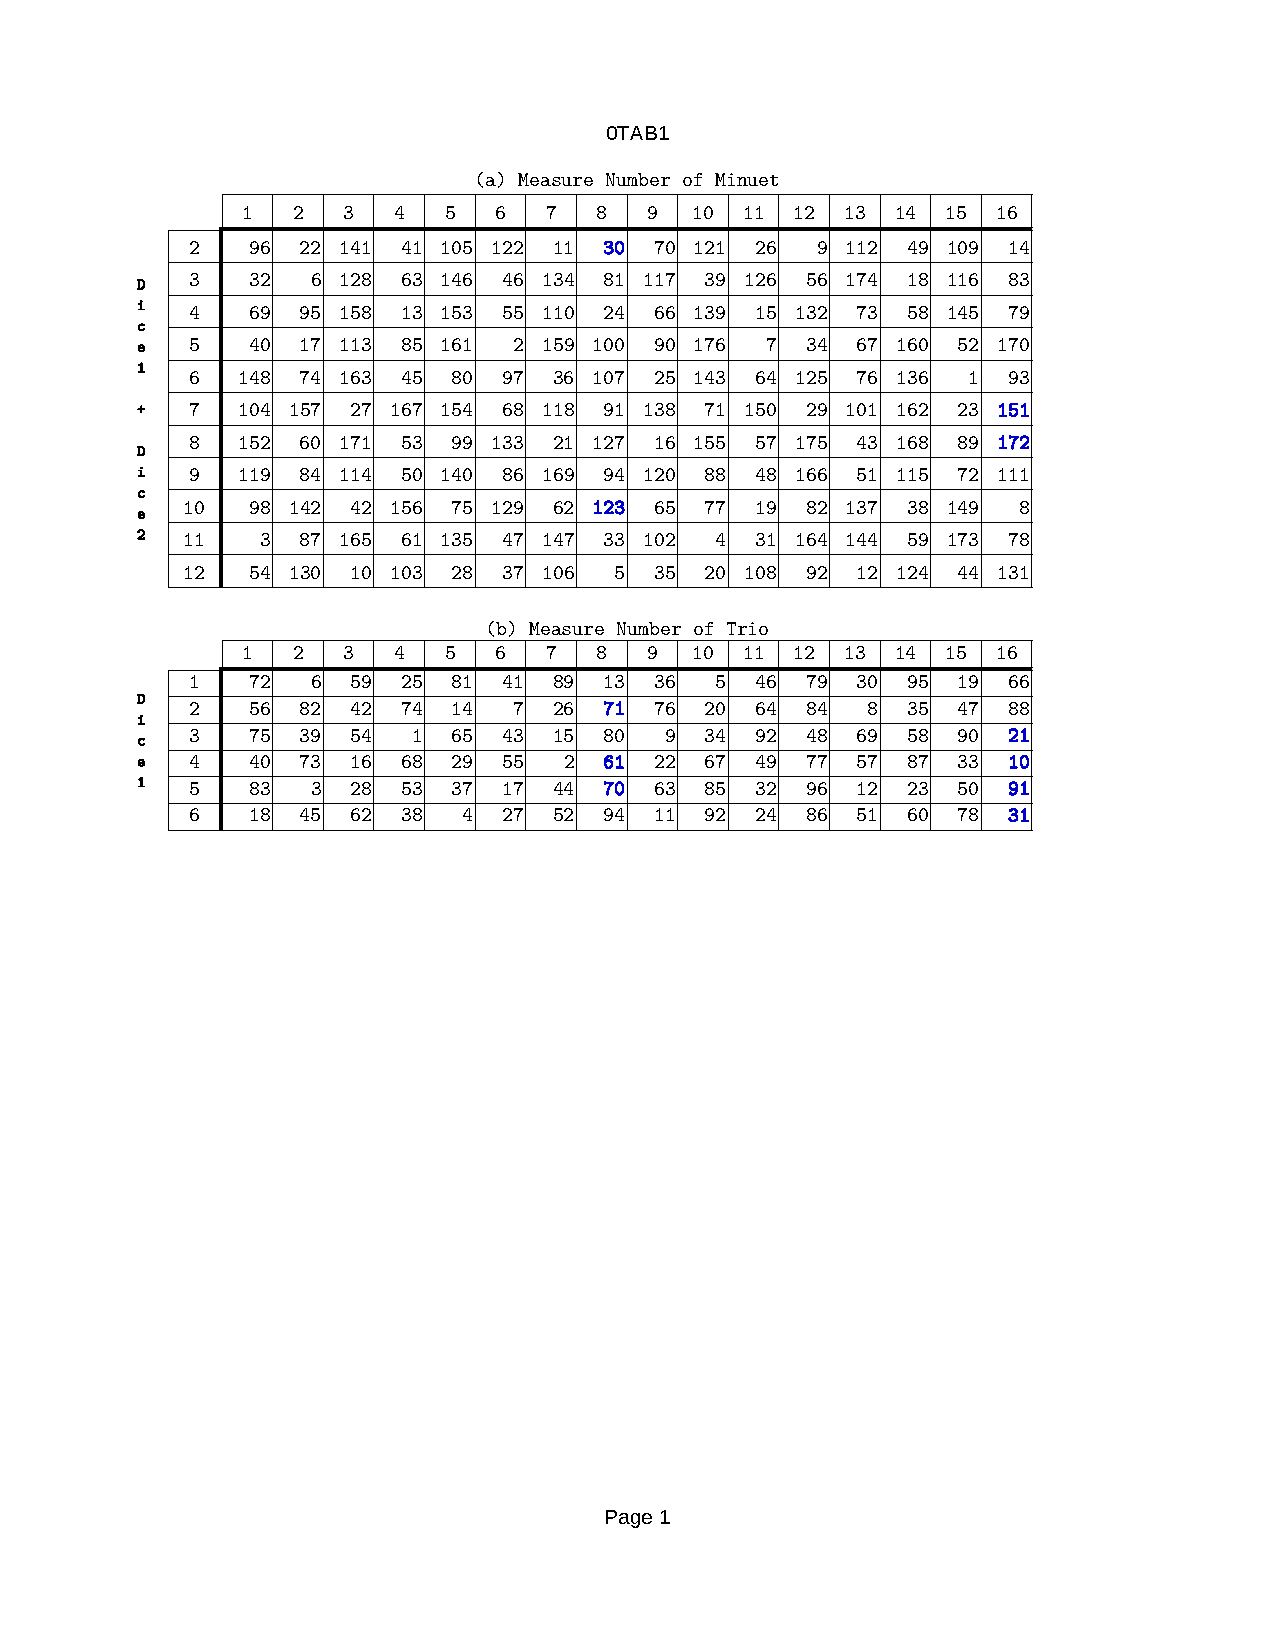
\includegraphics[clip=true,trim=0.90in 5.40in 1.25in 1.10in,scale=0.90]{gf-TAB}
	\end{tabular}
	\caption{Measure number to be looked-up in the Table of Measures (see Figures~\ref{fig:meas1}, \ref{fig:meas2}, \ref{fig:meas3}, \ref{fig:meas4}, and \ref{fig:meas5} in Section~\ref{tableMeas}) corresponding to each two-dice outcome per measure for the minuet and one-die outcome for the trio. Measure number in {\bf\color{blue}bold blue font} indicates identical measures under that column (see  \href{https://opus-infinity.org/dice_games/stadler_menuet_trio/tables/}{https://opus-infinity.org} for more info).}
	\label{fig:0tab1}
\end{table}

Although the body of Table~\ref{fig:0tab1}(a) includes $11\times 16 = 176$ measure numbers, the Table of Measures for Minuets (Figures~\ref{fig:meas1} to \ref{fig:meas3}) contains only 174 different measures.  This is so since in Table~\ref{fig:0tab1}, although 11 choices are listed below each column, two choices under bar 8 (choices 30 and 123) and also under bar 16 (choices 151 and 172)) lead to identical notes in the Table of Measures for Minuets, so that only 10 different bars are under each of these two (2) columns. Consequently, the total number of different measures for minuets is $11\times 14 + 10 + 10 = 174$. \\

For the table for trios (Table~\ref{fig:0tab1}(a)), $6\times 16 = 96$ measure numbers are listed but there are only $6\times 14 + 4 + 3 = 91$ unique measures.  This is so since under the column for bar 8 for trios, choices 71, 61, and 70 lead to the same set of notes in the Table of Measures for Trios (Figures~\ref{fig:meas4} to \ref{fig:meas5}).  Also, under column for bar 16 for trios, choices 21, 10, 91, and 31 also lead to the same set of notes in the Table of Measures for Trios.

\nopagebreak[4]
\subsection{Table of Measures}\label{tableMeas}

\addcontentsline{toc}{subsection}{\hspace*{0.25in} Gioco Filarmonico page 1 of measures}
\begin{figure}[H]
	\centering
	\def\svgwidth{0.975\columnwidth}
	\input{haydnGF-easy-minuet001.pdf_tex}
	\caption{Table of Measures for Minuets (Part I)}
	\label{fig:meas1}
\end{figure}

\newpage
${}_{}$\\
\vspace{0.10in}
\addcontentsline{toc}{subsection}{\hspace*{0.25in} Gioco Filarmonico page 2 of measures}
\begin{figure}[H]
	\centering
	\def\svgwidth{0.975\columnwidth}
	\input{haydnGF-easy-minuet002.pdf_tex}
	\caption{Table of Measures for Minuets (Part II)}
	\label{fig:meas2}
\end{figure}

\newpage
${}_{}$\\
\vspace{0.10in}
\addcontentsline{toc}{subsection}{\hspace*{0.25in} Gioco Filarmonico page 3 of measures}	
\begin{figure}[H]
	\centering
	\def\svgwidth{0.975\columnwidth}
	\input{haydnGF-easy-minuet003.pdf_tex}
	\caption{Table of Measures for Minuets (Part III)}
	\label{fig:meas3}
\end{figure}

\newpage
${}_{}$\\
\vspace{0.10in}
\addcontentsline{toc}{subsection}{\hspace*{0.25in} Gioco Filarmonico page 4 of measures}
\begin{figure}[H]
	\centering
	\def\svgwidth{0.975\columnwidth}
	\input{haydnGF-easy-trio001.pdf_tex}
	\caption{Table of Measures for Trios (Part IV)}
	\label{fig:meas4}
\end{figure}

\newpage
${}_{}$\\
\vspace{0.10in}
\addcontentsline{toc}{subsection}{\hspace*{0.25in} Gioco Filarmonico page 5 of measures}
\begin{figure}[H]
	\centering
	\def\svgwidth{0.975\columnwidth}
	\input{haydnGF-easy-trio002.pdf_tex}
	\caption{Table of Measures for Trios (Part V)}
	\label{fig:meas5}
\end{figure}

\newpage
\section{Related Links}
The following are very interesting sites in that they allow the online rendering of MDGs:
\begin{itemize}
	\item \href{https://opus-infinity.org}{Opus Infinity} - Collaborative work of Robbert Harms, Hein Moors, and Suus van Petegem whose goal is to unravel the mystery behind the tables used for generating MDGs.  Site visitors can generate MDGs based on works of Kirnberger, Mozart, Stadler/Haydn, Bach, and Gerlach.  Corresponding audio files ({\tt mid, ogg,} and/or {\tt mp3}) and image files ({\tt pdf} or {\tt png}) are also made available for listening, viewing, or downloading.
	
	\item  \href{http://sunsite.univie.ac.at/Mozart/dice/}{Mozart} - A site maintained by John Chuang that allows the site visitor to generate MDGs based on the work of Stadler/Haydn.
 	
	\item  \href{https://marian-aldenhoevel.de/mozart/}{Mozart} - A site maintained by Marian Aldenh\"{o}vel allows the visitor to generate a MDG (user-specified or randomly-generated) and the corresponding audio ({\tt midi, wav}) and image files ({\tt pdf, png}) based on {\em Musikalisches W\"{u}rferspiel, K.\ 516f}.
 	
 	\item \href{https://www.amaranthpublishing.com/MozartDiceGame.htm}{\tt mozart.zip} -  This is a Windows software ({\small\textcopyright} 1995 VisionSoft) by John Chuang and Stephen Goodwin that generates MDG based on input from user and is available for {\it free} from  \href{http://www.amaranthpublishing.com/MozartDiceGame.htm}{Amaranth Publishing}.  
 	
 	\item \href{(http://www.asahi-net.or.jp/\~rb5h-ngc/e/k516f.htm}{``Mozart - Musical Game in C K. 516f,"}	Mozart Studies Online - The site of Hideo Noguchi that offers an explanation linking {\em Musikalisches W\"{u}rferspiel, K.\ 516f}, and  {\em K.\ 294d (K.\ Anh.\ C 30.01)}. 
\end{itemize}

\section{Acknowledgments}
My sincerest gratitude to Chris Walshaw et al. for the \href{http://www.abcnotation.com/}{ABC music notation}; Jean-Francois Moine for \href{http://moinejf.free.fr/}{\tt abcm2ps} and the accompanying examples, templates, and pointers for the appropriate use of these resources; Guido Gonzato for the \href{http://abcplus.sourceforge.net/}{ABC Plus Project} and the \href{http://abcplus.sourceforge.net/#abcMIDI}{{\tt abcmidi} resources} available there, more especially for the ABC resource book {\em Making Music with ABC 2}; James R. Allwright and Seymour Shlien for \href{http://abc.sourceforge.net/abcMIDI}{\tt abcmidi} source and binaries; \href{https://artifex.com/}{Artifex, Inc.} for Ghostscript v.10.00.0 (includes the {\tt ps2pdf} converter); \href{https://www.inkscape.org/}{Inkscape v.1.2.2} for the tool for converting SVGs to PDFs for inclusion into \LaTeX\ documents; William Schelter for \href{https://maxima.sourceforge.io}{Maxima v.5.47.0}---used for computing the permutation number; and \href{https://tex.stackexchange.com/users/632/martin-h}{\tt User:Martin H} for his \href{https://tex.stackexchange.com/questions/2099/how-to-include-svg-diagrams-in-latex}{reply} to a TeX/LaTeX Stack Exchange question on including SVGs into \LaTeX\ documents. Special thanks also to the \href{http://imslp.org/}{International Music Score Library Project (IMSLP)} for making available the score for \href{http://imslp.org/wiki/Table\_pour\_composer\_des\_Minuets\_et\_des\_Trios\_\%C3\%A0\_la\_infinie\_(Stadler,_Maximilian)}{
Table pour composer des Minuets et des Trios à la infinie} and \href{https://www.amaranthpublishing.com/MozartDiceGame.htm}{Amaranth Publishing} for a copy of {\tt mozart.zip}. Ditto to Machtelt Garrels for the book \href{http://tldp.org/LDP/Bash-Beginners-Guide/html/Bash-Beginners-Guide.html}{Bash Guide for Beginners}, Vivek Gite for the book \href{http://www.freeos.com/guides/lsst/}{Linux Script Shell Tutorial}, and Steve Parker for the \href{http://steve-parker.org/sh/cheatsheet.pdf}{Unix/Linux Shell Cheatsheet}. John Fogarty's GitHub Site: \href{https://github.com/jfogarty/latex-createspace-bookcover}{Latex CreateSpace BookCover} and Peter Wilson's reply in TeX/LaTeX Stack Exchange on \href{https://tex.stackexchange.com/questions/17579/how-can-i-design-a-book-cover}{designing a book cover}, were sources of ideas, information, and materials for creating the book cover and title page, thanks to both of them; \href{http://www.libreoffice.org/}{LibreOffice Calc} for its use in the image creation of the book cover.  Many thanks, too, to the \href{https://www.debian.org}{Debian Project} for the Debian 12 (Bookworm) GNU/Linux OS, \href{http://www.tug.org/texlive/}{TeXLive 2024} for providing the \TeX\ distribution,  and \href{https://github.com}{GitHub} for its generosity in providing space for \href{https://github.com/justineuro/mdgBookSVGKit}{the project}.  

\newpage
\section{Selected Waltzes}
{
\topmargin -1.00in
\textheight 10.25in
	\input{svgList}
}	

\section{License}
This work by I Am The Author, based on work of J.L.A. Uro at  \url{https://github.com/justineuro/mdgBookSVG4Kit}, is licensed under a Creative Commons Public Domain International License.

%\bibliographystyle{plainnat}
%\bibliography{mdg4}

 

\end{document}
